\documentclass[12pt]{article}
\usepackage[letterpaper, margin=1in]{geometry}
\usepackage{graphicx}
\usepackage{amsmath}
\usepackage[framed, numbered]{matlab-prettifier}
\lstset{inputpath=../Matlab}
\graphicspath{{../Figures/}}
\title{ELECENG 3TP3 Lab 3}
\author{Raeed Hassan \\ hassam41 \\ McMaster University}
\begin{document}
\maketitle
\pagebreak
\section*{Aliasing in the Telephone System}
\begin{enumerate}
    \item
    A discrete time signal (an impulse train) resembling one period of a sine wave with a period of 10 ms can be seen when the the signal is plotted using the stem command. The graph can be seen in Figure~\ref{fig:tele_question1}.
    \begin{figure}[!ht]
        \centering
        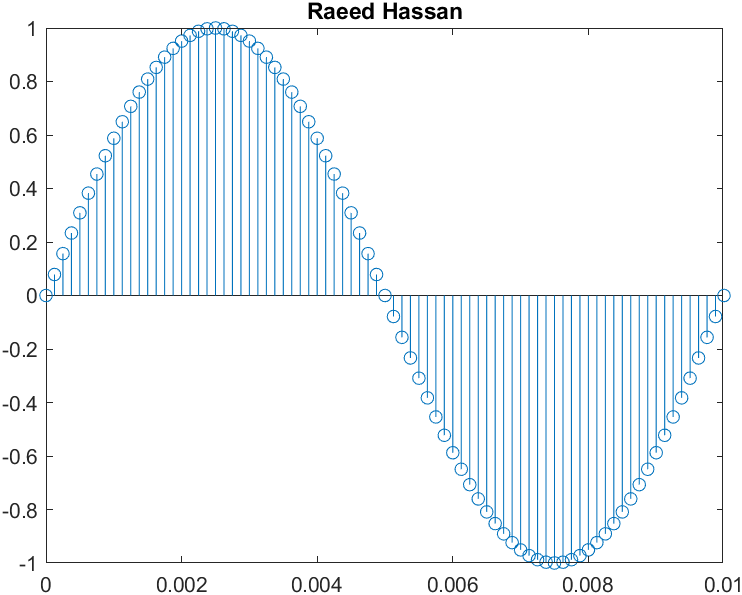
\includegraphics[width=\textwidth]{tele_question1}
        \caption{\label{fig:tele_question1}Question 1}
    \end{figure}
    
    \item
    The 8-second sound file begins with a relatively deep (low pitch/frequency) sound, with the sound increasing in pitch (frequency) every 2 seconds. In general, the higher frequency tone segments appear to sound louder than the lower frequency tone segments. The MATLAB code for generating the sound file and the plots is shown in Listing~\ref{listing:tele_question2}. The graph plotting all four output frequency plots is shown in Figure~\ref{fig:tele_question2}.
    \lstinputlisting[style=Matlab-editor, caption={Question 2}, label={listing:tele_question2}]{tele_question2.m}
    \begin{figure}[!ht]
        \centering
        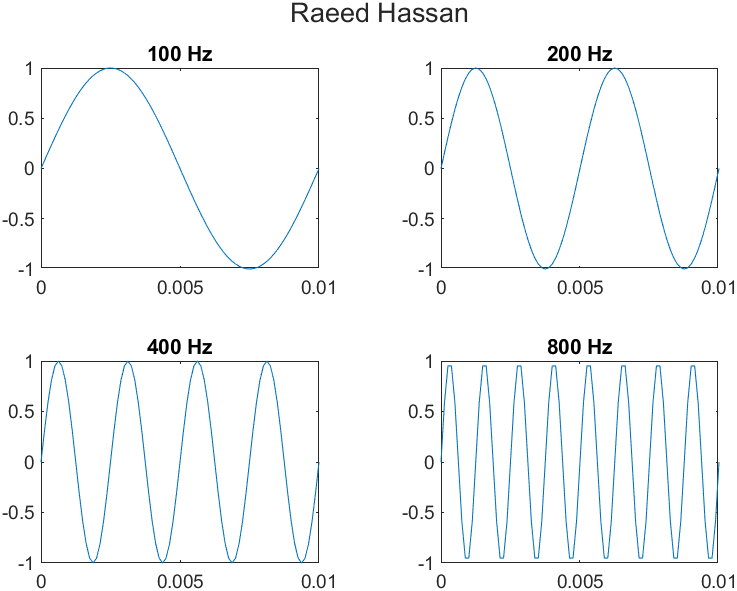
\includegraphics[width=0.62\textwidth]{tele_question2}
        \caption{\label{fig:tele_question2}Question 2}
    \end{figure}

    \item
    When the input frequencies were 7200, 7600, 7800, and 7900 Hz instead of the original 100, 200, 400 and 800 Hz, the observed output frequency of the sound does not display the intended effect. With the higher frequencies, the output sound file sounds like it starts at a higher frequency, and decreases in frequency every 2 seconds, when the opposite is true for the input frequencies. 
    
    As you keep increasing the frequency of the input sinusoid, it is possible to still hear the intended pattern, but the output frequencies are inconsistent and do not always match the patterns of the input frequencies. At multiples of 4000 Hz, at and over 8000 Hz, there is no sound produced. 
    
    This occurs because the the input frequencies require a sampling rate greater than 8 KHz (sampling rate must be twice the frequency of the input signal) or else information about the original signal will be lost due to aliasing. 

    \item
    The performance of the telephone system would degrade significantly if anti-aliasing pre-filtering were not used as sounds above 4 KHz that enter the system would not be correctly replicated at the destination, as information about the sound is lost due to an inefficient sampling rate. The sound at the output will not match expected behaviour of the original signal, and the perceived output frequencies at the destination may be drastically different from the original input frequency. For example, a high frequency sound could be perceived as a low frequency sound at the destination.
    
    Anti-aliasing pre-filtering prevents these negative effects by filtering out signals that cannot be replicated at the output by reducing their frequencies, only allowing signals that can be accurately convert and transmitted to enter the system. This means all signals that are outputted at the destination will exhibit their expected behaviour relative to other signals at different frequencies (higher input frequencies will be transmitted at a higher frequency at the output), however this effect will diminish as the frequency increases and very high frequency sounds will likely sound the same.

    If filtering was applied in the above experiments, then the output frequencies would always be increasing (if the input frequencies were increasing), however the differences between the output frequencies would diminish as the input frequencies increased until eventually beginning to sound the same.
\end{enumerate}

\clearpage
\section*{Aliasing of a Frequency Chirp Signal}
\begin{enumerate}
    \item
    The audio file started as a relatively high frequency sound that continuously increased in frequency until it could no longer be heard. The plot of the first 2000 samples of the signal is shown in Figure~\ref{fig:chirp_question1}. The period of the sampled signal looks to be decreasing (and frequency increasing) as time goes on. The MATLAB code can be seen in Listing~\ref{listing:chirp_question1}.
    \lstinputlisting[style=Matlab-editor, caption={Question 1}, label={listing:chirp_question1}]{chirp_question1.m}
    \begin{figure}[!ht]
        \centering
        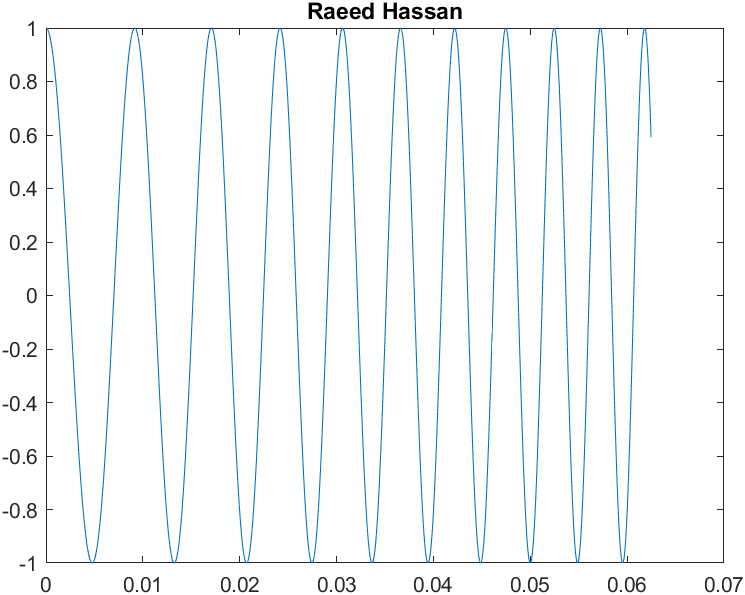
\includegraphics[width=0.64\textwidth]{chirp_question1}
        \caption{\label{fig:chirp_question1}Question 1}
    \end{figure}

    \item
    When the sampling frequency is set to 16 KHz, the sound begins to increase but takes approximately half the original time to become inaudible, then starts to decrease in frequency until stopping at around the beginning frequency. Due to an insufficient sampling frequency, the higher frequencies from the chirp signal produce a distorted output due to the higher frequencies not being sampled enough. 
    
    When the sampling is 8 KHz, the sound produced at 16 KHz is heard playing at twice the rate for the first half of the sound file, then repeats. If this signal were sent through the digital telephone network without anti-aliasing pre-filtering, the output as the destination would be exactly as heard in the sound file. If the telephone connection that includes the anti-aliasing filtering, then the sound would continuously increase in frequency at an increasingly lower rate of increase for the entire duration of the signal, until eventually becoming inaudible towards the end.
    
    The value of $f_1$ was experimented with $f_s = 32$ KHz and $\mu = 2000$. When the value of $f_1$ is increased, it produces a similar result as decreasing the value of $f_s$. The signal increases in frequency at a faster rate before beginning to decrease, then repeats the same pattern. The rate of increase will be larger as you increase the value of $f_1$. As the value of $f_1$ decreases, the rate of increase of the signal frequency appears to decrease. The output signals exhibit the expected behaviour as you change the value of $f_1$ (changes the frequency of the original signal) as long as the sampling frequency $f_s$ is sufficient.

    The value of $f_s$ was experimented with $f_1 = 100$ Hz and $\mu = 2000$. When the value of $f_s$ decreases, the signal appears to occur over a shorter duration and begins to repeat itself. The behaviour is likely due to the output signal becoming distorted as the sampling frequency decreases below the Nyquist sampling rate of the original signal.  When the value of $f_s$ increases, the signal appears to sound the same. This behaviour is due to the sampling frequency being sufficient for reproducing the input signal, and oversampling the original signal causing a minimal change in the output signal.

    The value of $\mu$ was experimented with $f_1 = 100$ Hz and $f_s = 32$ KHz. When the value of $\mu$ decreases, the rate of increase in the output frequency appears to decrease. When the value of $\mu$ increases, the rate of increase in the output frequency appears to increase, eventually causing the signal to repeat itself. This matches the behaviour of changing $f_1$, which is expected as the value of $\mu$ also changes the frequency of the the signal (at a rate that is proportional to the square of the change in $f_1$).  
\end{enumerate}
\end{document}